\section{Introduction}
\IEEEPARstart{W}{ith} this paper we hope to introduce an approach to effectively train a tracked robot to successfully navigate a foreign environment in order to retrieve and return an object. 

Currently for many tasks carried out by robots a human is required to control and monitor it's operation. This can be expensive and time consuming. However the human touch can be seen as necessary as humans have a better inherent ability to react to unplanned events in the environment.

Autonomous robotic navigation is not a novel concept however, and in recent years with the reduction in price of computing and increase in density of computing power many companies have successfully demonstrated autonomously navigating systems capable of reacting to a real-world environment. For example, Boston Dynamics have created their handle robot, capable of box handling in a warehouse \cite{BostonDynamics}. Or there's Tesla, who have created an autonomous self driving car \cite{Tesla}. 

The objective of this research is to present and evaluate an approach for training an Artificial Neural Network quickly and effectively on any platform it is presented with, so long as it's interactions are well defined. We hope this research will help tackle an issue with Neural Networks where they will be able to handle the environment they are trained in, and not work well beyond it. With faster training times 

This paper proposes our algorithm IOANNIS and hopes to demonstrate an adaptable approach to the development of a navigation system powered by Artificial Intelligence. It will be meant to be portable, meaning it can be trained on any device, and do so in a fast and efficient manner. The navigation system it produces should be able to avoid changing and moving obstacles in a foreign environment, while searching for an object it is meant to retrieve.

For the purpose of this research a simulation will be created using Unity, with the simulated robot being based on the IRIS robot (figure \ref{fig:irisImage}) provided by the University of Portsmouth.

\begin{figure}[h]
	\begin{center}
		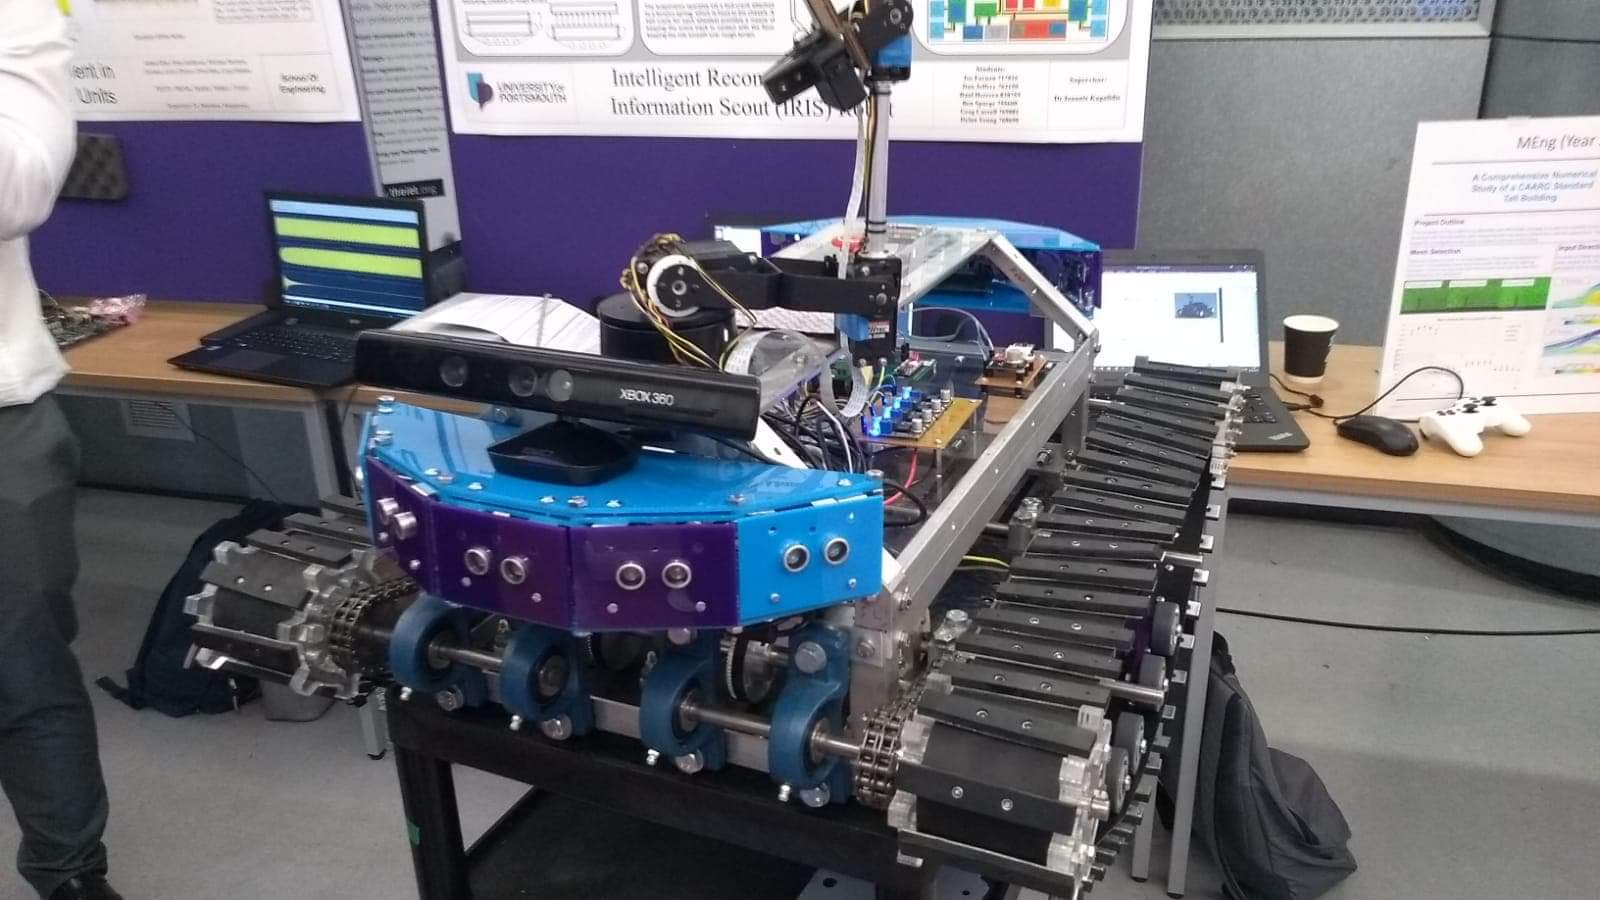
\includegraphics[width=1\linewidth]{iris}
		\caption{Iris Robot}
		\label{fig:irisImage}
	\end{center}
\end{figure}

The rest of this paper will be organised as follows. Related work will be critically reviewed in section II. Section III will discuss the design of the algorithm IOANNIS. Section IV will discuss the implementation of the algorithm. Experimental results will be presented in section V. Lastly, section VI will present our findings and conclusions, as well as propose areas for future work.